\documentclass[a4paper,12pt]{article}
\usepackage[utf8]{inputenc}
\usepackage{color}
\usepackage{url}
\usepackage{graphicx}
 
\title{Two Electron Matrix Elements in Coupled Spherical Harmonics}
\author{Tore Birkeland and Raymond Nepstad}

\newcommand{\bra}[1]{\ensuremath{\langle #1 |}}
\newcommand{\ket}[1]{\ensuremath{| #1 \rangle}}
\newcommand{\innerprod}[2]{\langle #1 | #2 \rangle}
\newcommand{\matelem}[3]{\langle #1 | #2 | #3 \rangle}
\newcommand{\cg}[6]{\innerprod{#1 #2 #3 #4}{#5 #6}}
\renewcommand{\imath}{{\mathrm i}}
\newcommand{\partialdiff}[2]{\frac{\partial #1}{\partial #2}}
\renewcommand{\vec}[1]{\ensuremath{\textbf{#1}}}


\begin{document}

\section{Testing the e-e term}
Calculation of bound state energies is a good test of the correctness and accuracy of the electron-electron interaction term. We have tried three different eigenvalue methods: direct (SciPy), Jacobi-Davidson (Pysparse) and preconditioned Arnoldi Shift-Invert iterations (PyProp, PIRAM+GMRES+PRECON). We have tested all three for $L=0$, and they gave the same results (to requested precision).

\begin{itemize}
	\item $r_{max}$ = 200
	\item Number of breakpoints: 30
	\item Exponential breakpoint sequence, $\gamma = 7.0$
	\item $l_{max} = 5$, all terms for given $L$ and $M$ are included
	\item Extra integration points: 20
\end{itemize}

\begin{table}
\centering
\begin{tabular}{lccc}
	\hline\\
	Helium state & Our & Hasbani \textit{et. al.} & Other\\
	\hline\\
	$^1S^e(1)$ & -2.903\ 586 (JD) & -2.903\ 531 & -2.903\ 724\\
	$^1S^e(2)$ & -2.145\ 965 (JD) & -2.145\ 961 & -2.145\ 974\\
	$^1S^e(3)$ & -2.061\ 270 (JD), & -2.061\ 268 & -2.061\ 272\\
	$^1S^e(4)$ & -2.033\ 586 (JD) & -2.033\ 585 & -2.033\ 586\\
	\\
	$^1P^o(1)$ & -2.123\ 829 (JD) & -2.123\ 832 & -2.123\ 843\\
	$^1P^o(2)$ & -2.055\ 142 (JD) & -2.055\ 143 & -2.055\ 146\\
	\\
	$^1D^e(1)$ & -2.055\ 636 (ASI) & -2.055\ 621 & -2.055\ 621\\
	$^1D^e(2)$ & -2.031\ 280 (ASI) & -2.031\ 280 & -2.021\ 279\\
	\\
	$^1F^o(1)$ & -2.031\ 255 (JD) & -2.031\ 255 & -2.031\ 255\\
	$^1F^o(2)$ & -2.020\ 003 (JD)& -2.020\ 003 & -2.020\ 033\\
	$^1F^o(3)$ & -2.013\ 891 (JD) & -2.013\ 891 & -2.013\ 891\\
	$^1F^o(4)$ & -2.010\ 205 (JD) & -2.010\ 205 & -2.010\ 205\\
\end{tabular}
\caption{Helium bound state energies (a.u.). JD: Jacobi-Davidson, ASI: Arnoldi Shift-Invert iterations}
\label{tab:}
\end{table}

\section{Testing the laser potential term}
It is not so easy to verify correctness for time-dependent potential terms. The best we can do is to compare with a test case from the litterature. We have selected some results from Hasbani \textit{et. al.} [ref], which we will attempt to reproduce.
%
B-spline parameters
\begin{itemize}
	\item $r_{max}$ = 100
	\item Number of breakpoints: 65
	\item Exponential-linear breakpoint sequence, $\gamma = 3.0$ and $r_c = 20$.
	\item $l_{max} = 5$, $L_{max} = 5$, $M = 0$.
\end{itemize}
%
Pulse parameters
\begin{itemize}
	\item $T_{pulse}$ = 3.8 fs
	\item Peak intensity = 2.96 W/cm$^2$
	\item cos$^2$ envelope
	\item Frequency range: 0.2 - 1.2
\end{itemize}

To calculate ionization+excitation, we simply project on the intial state. Ionization is determined by removing from the final wavefunction population in all states of energy less the the single ionization threshold (-2.0 a.u.). These states were determined from the above-mentioned Arnoldi Shift-Invert method.

\begin{figure}[ht]
\begin{center}
	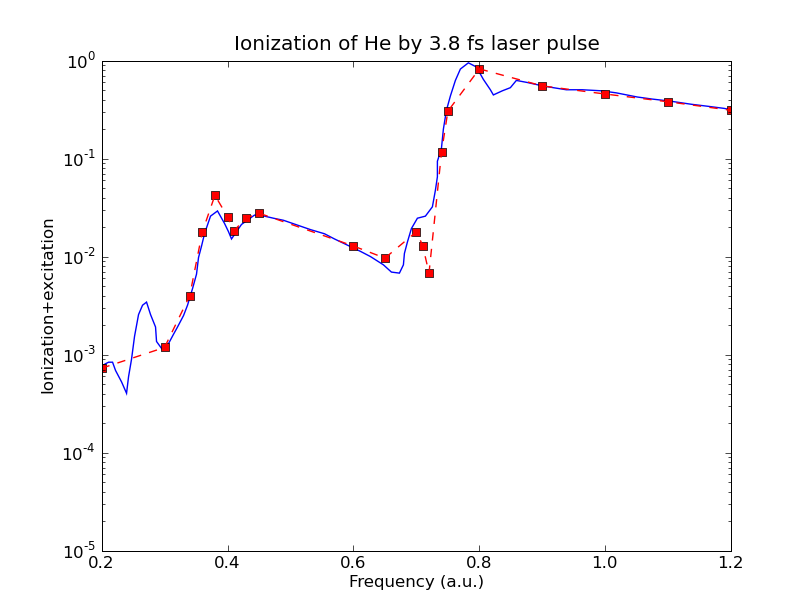
\includegraphics[width=\textwidth]{hasbani_pyprop2e_ionization_excitation.png}
\end{center}
\caption{Ionization+excitation.}
\end{figure}

\begin{figure}[ht]
\begin{center}
	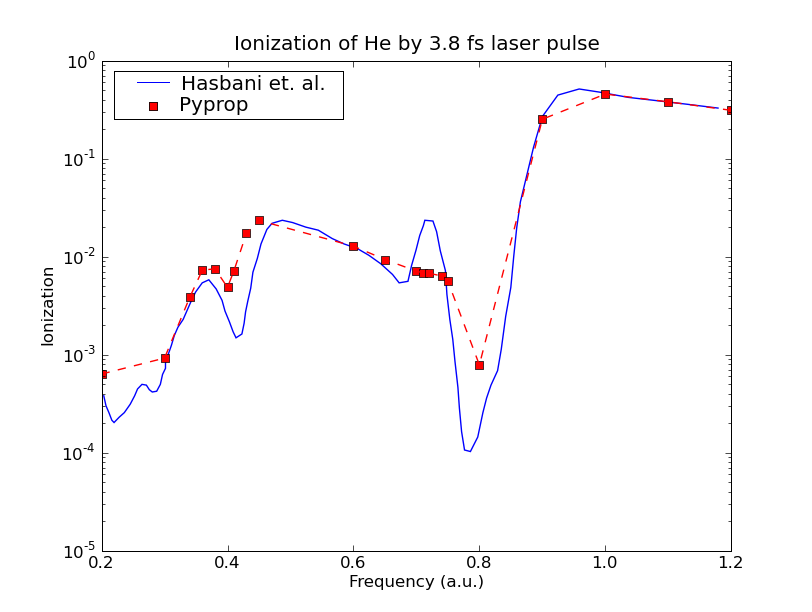
\includegraphics[width=\textwidth]{hasbani_pyprop2e_ionization.png}
\end{center}
\caption{Ionization.}
\end{figure}


\end{document}
